\documentclass[11pt]{article}

\usepackage{microtype}
\usepackage{graphicx}
\usepackage{booktabs}
\usepackage{array}
\usepackage{amsmath}
\usepackage{amsfonts}
\usepackage{amssymb}
\usepackage{enumitem}
\usepackage{tikz}
\usetikzlibrary{positioning,decorations.pathreplacing}
\usepackage{microsoft-tech-report}
\usepackage{hyperref}
\usepackage{xeCJK}
\setCJKmainfont{FandolSong}[ItalicFont=FandolKai]
\setCJKsansfont{FandolHei}
\setCJKmonofont{FandolFang}
\xeCJKsetup{BoldFont={*}}

% \newcommand{\add}[1]{{\color{blue}#1}}
\newcommand{\add}[1]{{#1}}
\newcommand{\harl}{脚手架驱动的智能体强化学习}
\newcommand{\Harl}{脚手架驱动的智能体强化学习（Harnessed Agentic RL）}

\hypersetup{
  colorlinks=true,
  linkcolor=microsoftblue,
  citecolor=microsoftblue,
  urlcolor=microsoftblue,
  pdftitle={Agent Lightning v1.0: Towards Harnessed Agentic RL},
  pdfauthor={First Author, Second Author},
  pdfsubject={Technical report},
  pdfkeywords={technical report, latex template}
}

\techreportlabel{Agent Lightning v1.0：迈向\add{\Harl{}}}
\techreportshorttitle{Agent Lightning v1.0：迈向\add{\Harl{}}}
\techreportlogoheight{0.75cm}
\newcommand{\reportkeywords}{technical report, latex template, reproducible research}
\renewcommand{\techreportmonthyear}{2026年8月}

\begin{document}
\thispagestyle{empty}
\enlargethispage{1.0cm}

\techreportlogos{%
  \techreportlogo{figures/microsoft.pdf}
}%
\techreportdate{\techreportmonthyear}
\techreporttoprule

\techreporttitle{\fontsize{17}{17}\selectfont Agent Lightning v1.0：迈向\add{\Harl{}}}
\techreportauthors{%
  Zhiyuan He$^{1,*,\ddagger}$ \hspace{0.7em}
  Siwei Zhang$^{2,*}$ \hspace{0.7em}
  Zhiwen Zhou$^{3,*}$ \hspace{0.7em}
  Yuqing Yang$^{1,\ddagger}$ \hspace{0.7em}
  Yu Kang$^{1}$ \hspace{0.7em} \\
  Yuge Zhang$^{1}$ \hspace{0.7em}
  Luna K. Qiu$^{1}$ \hspace{0.7em}
  Tin Yan Tsui$^{4}$ \hspace{0.7em}
  Jiahang Xu$^{1}$ \hspace{0.7em}
  Chong Luo$^{1}$
}{%
  $^{1}$微软 \quad
  $^{2}$复旦大学 \quad
  $^{3}$浙江大学 \quad
  $^{4}$爱丁堡大学
}

\begin{center}
\begin{minipage}{\textwidth}
  \centering
  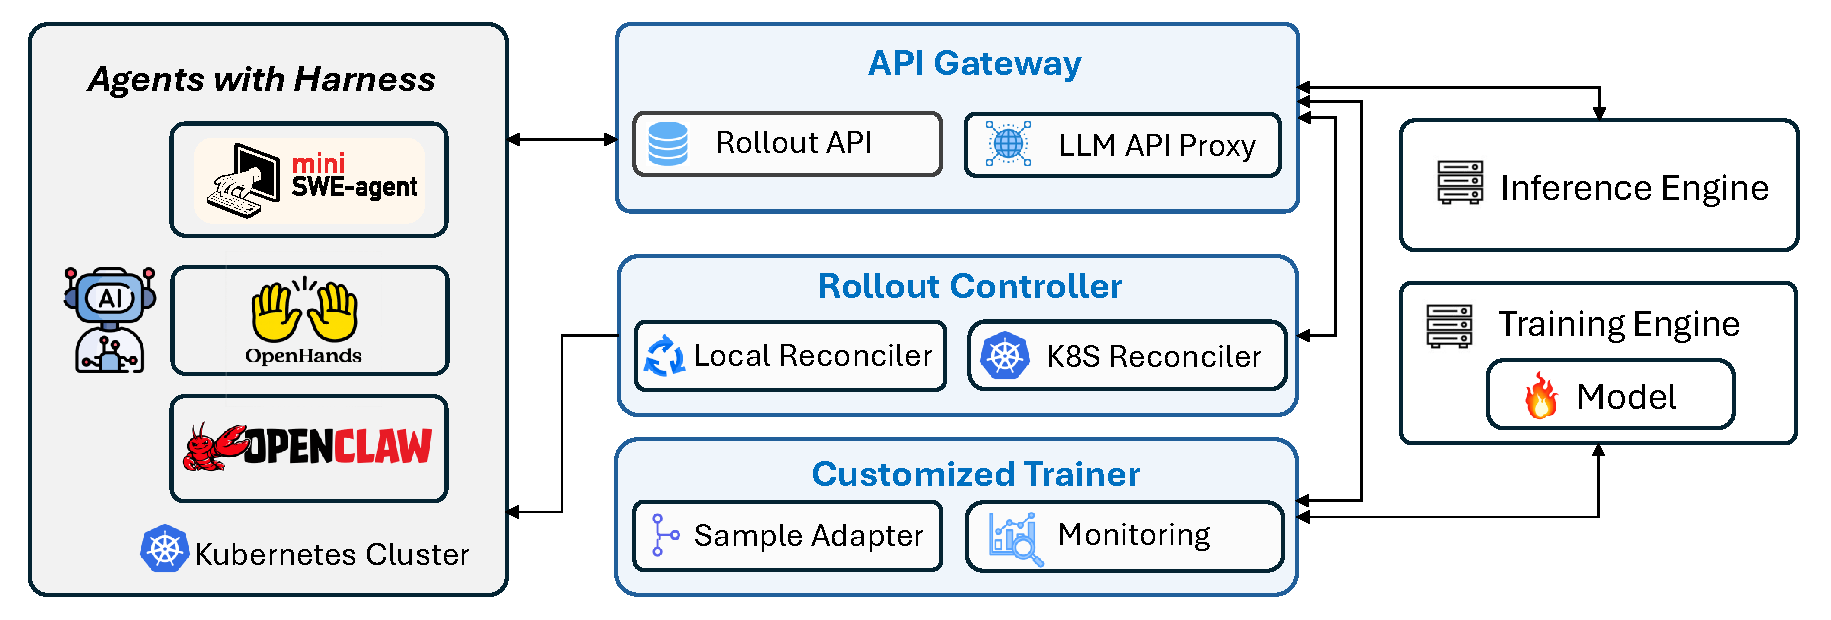
\includegraphics[width=\textwidth]{figures/agl-lite-teaser-0814.pdf}
  {\captionsetup{font=scriptsize,aboveskip=0pt,belowskip=0pt}
  \captionof{figure}{Agent Lightning v1.0 的整体框架。}
  \label{fig:teaser}}
\end{minipage}
\end{center}

\vspace{-0.2em}
\begin{microsofttitlebox}
\setlength{\parindent}{0cm}
\setlength{\parskip}{0.02cm}
\raggedright
\nohyphens

\begin{abstract}
\textbf{摘要。}
现代智能体并非独立运行的 LLM。它们运行在管理工具、上下文与控制流的\emph{智能体脚手架（agent harness）}之中，脚手架因此成为智能体的关键组成部分。我们最初的 Agent Lightning 工作提出了训练与智能体执行解耦的架构，通过 LLM 端点代理将任意智能体接入强化学习（RL）训练。近期的框架如 verl Uni-Agent、AReaL 2.0、slime v0.3.0 与 Polar 均沿用了这种基于代理的方式，使 RL 训练得以在脚手架中进行。本文将这一范式称为\emph{\add{\harl{}}}（Harnessed Agentic RL）：部署时脚手架直接参与模型后训练，从而缩小训练与实际使用之间的差距。

\vspace{\baselineskip}

我们发现\add{\harl{}}与传统智能体 RL 有本质区别，并带来一系列新挑战。传统智能体 RL 中，训练引擎拥有环境交互循环；而在\add{\harl{}}中，脚手架拥有这一循环，训练引擎只能观察到一串 LLM 请求-响应对。如何建模并将这些调用组装成训练样本仍是一个开放问题。通过仔细研究，我们识别出\harl{}的若干挑战，包括重分词、样本合并、优势计算、损失归一化与训练后端调度。我们发现，若处理不当，这些挑战会导致训练无效或不稳定。现有框架普遍对此语焉不详。本文首次对这些挑战给出系统性阐述。

\vspace{\baselineskip}

我们进一步提出 Agent Lightning v1.0，一个面向\add{\harl{}}的轻量级框架。我们将简洁作为第一原则，整个框架\textbf{仅用约 3500 行代码实现}。其紧凑设计支持任意智能体脚手架，并为研究上述挑战提供实用的试验平台。我们在通用指令遵循智能体、搜索智能体与编程智能体上验证了 Agent Lightning v1.0。对于编程智能体，我们发现现有 RL 框架支持有限：缺少数据与完整训练脚本，且依赖大规模计算资源。为填补这一空白，我们基于开源数据集与模型提供了完整的数据清洗管线与可复现的训练脚本。\textbf{仅使用 6K 训练样本与适量算力，RL 将 Qwen3.5-9B 在 SWE-bench Verified 上从 41.8\% 提升至 56.4\%，绝对提升 14.6\%。}我们发布完整工作流与脚本，以促进可复现的\add{\harl{}}研究。
\vspace{\baselineskip}

\end{abstract}


\vspace{0.08cm}
{\setlength{\parskip}{0.1cm}\scriptsize
\techreportmeta{项目主页}{\href{https://github.com/microsoft/agent-lightning}{github.com/microsoft/agent-lightning}}
\techreportmeta{通讯作者}{%
\href{mailto:zhiyuhe@microsoft,yuqyang@example.com}{\{zhiyuhe, yuqyang\}@microsoft.com}}
% \techreportmeta{Keywords}{\reportkeywords}
% \techreportmeta{Date}{\techreportmonthyear}
}
\vspace{0.08cm}
{\footnotesize\rmfamily\itshape\color{microsoftgray}
$^*$同等贡献。\quad
$^{\ddagger}$通讯作者。\par
}
\end{microsofttitlebox}

\clearpage
\section{引言}

现代智能体并非独立运行的 LLM。它们运行在管理工具、执行环境、上下文与控制流的\emph{智能体脚手架（agent harness）}之中。脚手架因此决定了智能体如何观察环境、如何长程行动、如何从失败中恢复，是智能体能力的核心部分。典型例子包括 mini-SWE-agent~\cite{minisweagent}、OpenHands~\cite{openhands}、OpenCode~\cite{opencode}、Claude Code~\cite{claudecode}、Codex~\cite{codex} 等编程智能体脚手架，以及 OpenClaw~\cite{openclaw}、Hermes~\cite{hermes} 等通用脚手架。

早期强化学习（RL）框架，如 verl~\cite{hybridflow}、AReaL~\cite{areal} 与 slime~\cite{slime}，通常要求用户直接在训练框架内部实现智能体循环。由于现有智能体脚手架实现复杂、依赖自成体系，将其直接集成进 RL 框架十分困难。我们最初的 Agent Lightning~\cite{agentlightning} 工作提出了训练与智能体执行解耦的架构，通过 LLM 端点将任意智能体接入 RL 训练，几乎无需改动智能体本身。近来，这种基于代理的方式已被 verl Uni-Agent~\cite{uniagent}、AReaL 2.0~\cite{areal2}、slime v0.3.0~\cite{slime} 与 Polar~\cite{polar} 等框架广泛采用，自然支持在智能体脚手架上进行 RL 训练。

\add{本文将“通过部署时的同一智能体脚手架进行 RL 训练”这一范式称为\emph{\harl{}}。由脚手架——而非训练器——拥有上下文构建、工具执行与智能体-环境交互循环，训练系统则跨越服务边界观察并优化由此产生的模型调用。这种形式保留了脚手架部署时的上下文策略、工具协议与执行语义，无需在 RL 框架内部重新实现其智能体循环。}

\add{传统智能体 RL 与\harl{}都可以建模为部分可观测马尔可夫决策过程（POMDP），但二者的潜在状态与呈现给策略模型的观测不同。传统智能体 RL 中，潜在状态主要是环境状态，策略模型通过透明层几乎直接与环境交互：模型生成动作 token，环境返回观测，token 化后的观测扩展已有历史，
$p_t = \bigl(p_{t-1},a_{t-1},o_t\bigr)$。
其中 $p_t$ 为第 $t$ 步呈现给模型的 token 历史，$a_{t-1}$ 为上一步生成的动作，$o_t$ 为最新的环境观测。因此策略观察到的是连续扩展的 token 历史，一次 rollout 自然构成一条线性 token 轨迹。

在\harl{}中，策略模型不再直接与环境交互。潜在状态同时包含脚手架状态与环境状态。脚手架拥有上下文构建、控制流、工具执行与智能体编排，并为每次模型调用独立构造请求 prompt。策略只能观察到经 LLM API 送达的确切 prompt，并基于该 prompt 生成响应。因此，一次 rollout 在模型边界上呈现为一串请求-响应对，
\[
  (p_1,a_1),(p_2,a_2),\ldots,
\]
其中 $p_i$ 为第 $i$ 次 LLM 调用发送的 prompt，$a_i$ 为对应的模型响应。介于其间的脚手架与环境状态转移保持潜在。图~\ref{fig:agentic-harness-centric-comparison} 总结了这一差异。这种差异也带来了下述实现挑战——现有框架对这些挑战的不同处理方式，可能影响算法正确性与训练稳定性。}

\begin{figure*}[t]
  \centering
  \begin{minipage}[c]{0.55\textwidth}
    \centering
    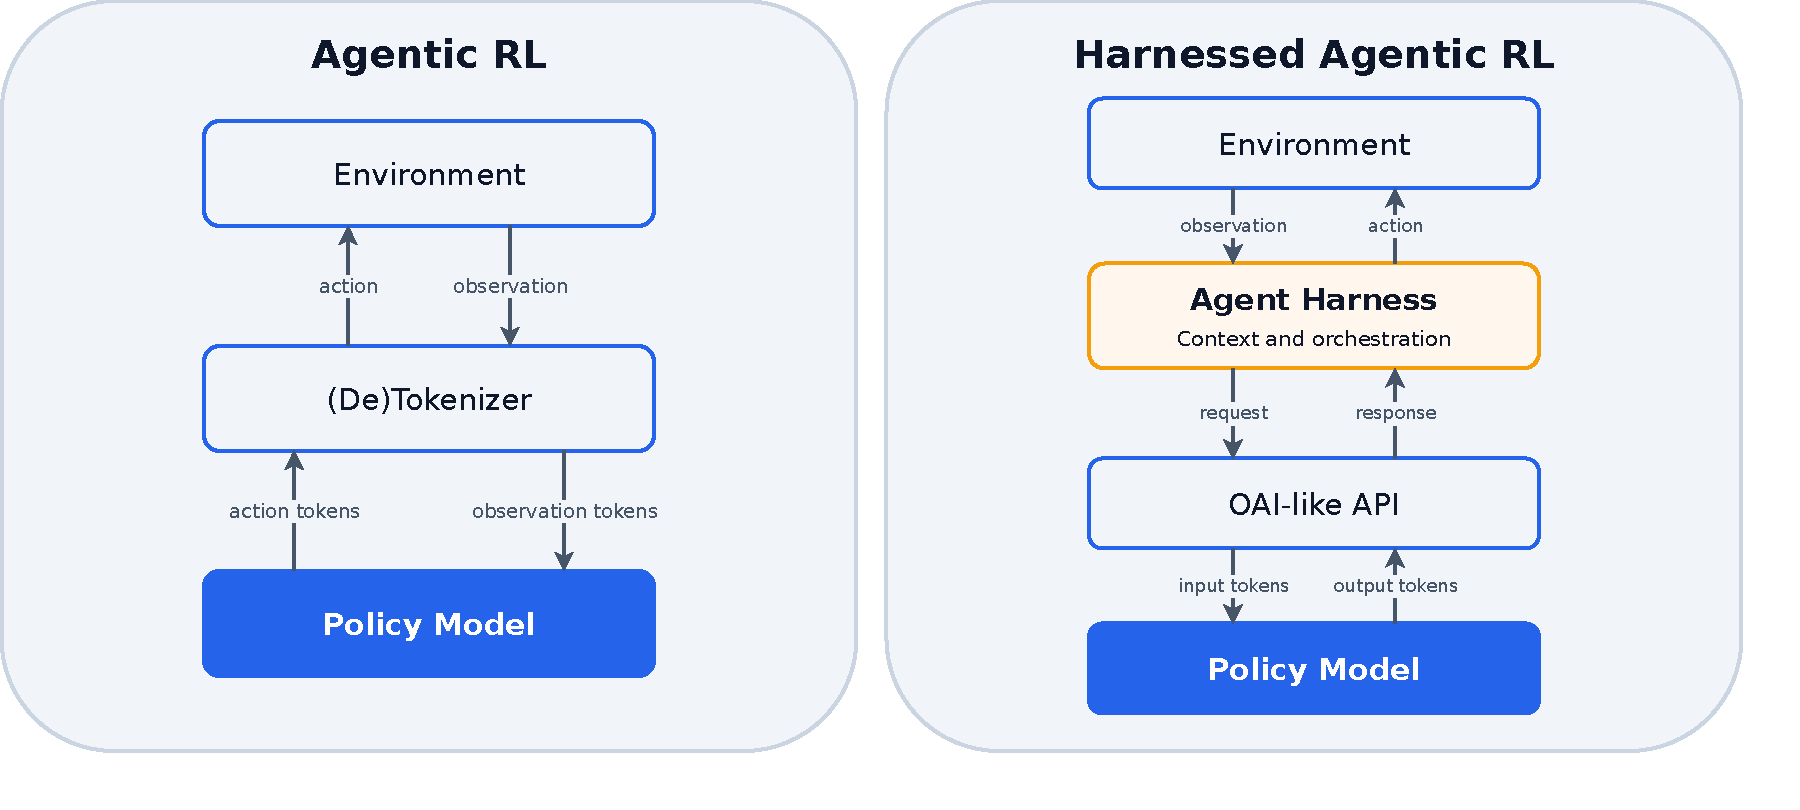
\includegraphics[width=\linewidth]
      {figures/agentic-harness-centric-comparison.pdf}
  \end{minipage}\hfill
  \begin{minipage}[c]{0.43\textwidth}
    \centering
    \scriptsize
    \setlength{\tabcolsep}{2pt}
    \renewcommand{\arraystretch}{1.06}
    \begin{tabular}{@{}
      >{\raggedright\arraybackslash}p{0.16\linewidth}
      >{\raggedright\arraybackslash}p{0.33\linewidth}
      >{\raggedright\arraybackslash}p{0.45\linewidth}@{}}
      \toprule
      & \textbf{智能体 RL} & \textbf{\add{\Harl{}}} \\
      \midrule
      \textbf{状态} &
        环境 &
        脚手架 + 环境 \\
      \hline
      \textbf{模型输入} &
        连续 token 历史 &
        每次调用独立 prompt \\
      \hline
      \textbf{智能体} &
        单一 ReAct 智能体 &
        多智能体、子智能体与交接 \\
      \bottomrule
    \end{tabular}
  \end{minipage}
  \caption{\add{传统智能体 RL 与\harl{}的对比。二者都可用 POMDP 刻画，但\harl{}在潜在执行状态中加入脚手架状态，并向策略模型暴露独立构造的模型调用 prompt。这一变化还将控制与编排移入脚手架，并使训练样本数量更加动态。}}
  \label{fig:agentic-harness-centric-comparison}
\end{figure*}

\textbf{第一个挑战是重分词与样本合并。}智能体脚手架通常通过文本消息与模型 API 通信，而 RL 训练在 token 上操作。多数框架在 $p_{i+1}$ 于 token 层面完整包含 $(p_i,a_i)$ 前缀时合并两次相邻调用。然而，重分词之后，即使文本不变，$p_{i+1}$ 中 $a_i$ 的 token ID 也可能与模型最初采样时不同。这破坏了 token 级连续性，使两次调用无法安全合并。

\textbf{第二，优势计算。}传统智能体 RL 中，每次 rollout 是一个马尔可夫过程，映射到唯一的训练样本。在\add{\harl{}}中，一次 rollout 可能产生动态数量的训练样本，原因不仅包括上述重分词问题，还包括脚手架派生子智能体、摘要压缩上下文等操作。这些动态样本给奖励与优势如何分配到训练样本带来了挑战。

\textbf{第三是损失归一化。}在\add{\harl{}}中，一次 rollout 可能映射到多个训练样本，使每个训练批次中的样本数量动态变化，损失归一化因此变得不平凡。例如，部分现有框架仍在样本层面归一化损失，使产生更多样本的 rollout 获得更大的优化权重，可能导致训练不稳定。

\textbf{第四是动态样本数量下的训练后端调度。}一批 rollout 产生的样本数量只有在脚手架执行与样本构建之后才能确定，而训练 GPU 数量及其并行配置保持固定。后端必须将变化的样本集切分为训练步与小批次，同时在固定的 GPU worker 之间均衡负载。

本文首次系统刻画了这些挑战，并进一步提出 Agent Lightning v1.0——对原始 Agent Lightning 的全面重构。它是一个面向任意智能体脚手架的轻量级 RL 训练框架。我们的设计原则是尽可能保持系统简单，仅用约 3500 行代码实现。其训练管线也内置了我们针对上述挑战的设计选择，为研究这些挑战提供了实用的试验平台。

我们使用 Agent Lightning v1.0 训练通用指令遵循智能体、搜索智能体与编程智能体。尤其地，现有智能体框架对编程智能体支持有限：缺少数据与完整训练脚本，可能源于数据清洗复杂、环境搭建困难与所需算力巨大。为填补这一空白，我们基于开源 SWE-smith 数据集与 Qwen3.5-9B~\cite{qwen35} 提供完整的数据清洗管线与可复现训练脚本。我们最终的 RL 训练仅使用 6K 训练样本与适量算力。\add{仅靠 RL，训练后的模型在 SWE-bench Verified 上从 41.8\% 提升至 56.4\%，绝对提升 14.6\%。}我们向社区发布完整工作流与脚本，以促进可复现性。

\section{挑战}
\label{sec:challenges}

脚手架驱动的智能体强化学习改变了训练引擎观察与建模一次 rollout 的方式。在传统智能体 RL 中，训练引擎拥有环境交互循环并维护完整的 token 历史。此处 $p_t$ 表示第 $t$ 步的 prompt token，$a_t$ 表示对应的响应 token，$o_t$ 为 token 化的环境观测。下一步 prompt 构造为
\begin{equation}
  p_t = (p_{t-1},a_{t-1},o_t).
\end{equation}
整个 rollout 遵循序列 $(p_1,a_1,o_1,a_2,o_2,a_3,\ldots)$，构成良定义的马尔可夫过程，自然映射为一条线性训练样本。

在\add{\harl{}}中，脚手架拥有环境交互循环与消息状态，训练引擎只能观察通过 LLM 端点发出的调用。对一次 rollout $\rho$，它记录序列
\begin{equation}
  \mathcal{C}(\rho)
  = \bigl((p_1,a_1),(p_2,a_2),\ldots,(p_{T_\rho},a_{T_\rho})\bigr),
\end{equation}
其中 $p_i$ 为 prompt token，$a_i$ 为模型实际采样的响应 token。这些调用之间的环境交互与脚手架状态转移不可直接观察。因此，将观察到的调用序列组装为训练样本本身成为一个建模问题。这一差异带来了若干实现挑战。现有框架的处理方式各不相同，可能影响算法正确性与训练稳定性。

\add{更形式化地说，传统智能体 RL 与\harl{}都可用部分可观测马尔可夫决策过程（POMDP）刻画，区别在于潜在状态与呈现给策略模型的观测。在\harl{}中，令
\begin{equation}
  s_t = \bigl(s_t^{\mathrm{harness}},s_t^{\mathrm{env}}\bigr)
\end{equation}
表示由脚手架与环境共同维护的潜在执行状态。模型不直接观察 $s_t$；脚手架构造消息级上下文并将其渲染为用于生成的确切 token 级 prompt：
\begin{align}
  C_t^{\mathrm{msg}}
    &= \operatorname{Context}_{H}\bigl(s_t^{\mathrm{harness}}\bigr),\\
  p_t^{\mathrm{tok}}
    &= \operatorname{Tok}\bigl(\operatorname{Template}
       (C_t^{\mathrm{msg}})\bigr).
\end{align}
每个策略决策因此被记录为一次调用级转移
\begin{equation}
  z_t = \bigl(p_t^{\mathrm{tok}},a_t^{\mathrm{tok}}\bigr),
  \qquad
  a_t^{\mathrm{tok}} \sim
  \pi_\theta\bigl(\cdot \mid p_t^{\mathrm{tok}}\bigr).
\end{equation}
一次 rollout 产生变长集合的此类转移，且不假设相邻 prompt 之间存在精确的 token 前缀关系。任何为训练所做的序列构造都必须保留每个动作实际采样时所依据的 prompt。下面描述\harl{}特有的若干新挑战。}

\subsection{重分词与样本合并}

\paragraph{\add{为什么 token 前缀连续性会被破坏。}}

\begin{figure}[t]
  \centering
  \begin{tikzpicture}[
      tok/.style={draw, rounded corners=1pt, minimum height=0.55cm,
        inner sep=2pt, font=\scriptsize, align=center},
      ptok/.style={tok, fill=microsoftcard, draw=microsoftline,
        text width=1.3cm},
      newtok/.style={tok, fill=microsoftcard, draw=microsoftline,
        text width=1.5cm},
      atok/.style={tok, fill=microsoftblue!12, draw=microsoftblue},
      mismatch/.style={tok, fill=red!12, draw=red!70!black},
      rowlabel/.style={font=\scriptsize\bfseries, text=microsoftgray,
        align=left, text width=3.1cm},
    ]
    \node[rowlabel] (labelA) at (0,1.7) {第 $i$ 次调用的实际采样};
    \node[ptok] (pA) at (3.3,1.7) {$p_i^{\mathrm{tok}}$};
    \node[atok, right=1mm of pA] (a1A) {h};
    \node[atok, right=1mm of a1A] (a2A) {aving};
    \draw[decorate, decoration={brace, amplitude=3pt, mirror},
      microsoftblue, thick]
      (a1A.south west) -- (a2A.south east)
      node[midway, yshift=-0.32cm, font=\scriptsize, text=microsoftblue]
      {$a_i^{\mathrm{tok}}$};

    \node[rowlabel] (labelB) at (0,0.3) {$p_{i+1}^{\mathrm{tok}}$ 的直接重分词};
    \node[ptok] (pB) at (3.3,0.3) {$p_i^{\mathrm{tok}}$};
    \node[mismatch, right=1mm of pB] (b1) {hav};
    \node[mismatch, right=1mm of b1] (b2) {ing};
    \node[newtok, right=1mm of b2] (bnew) {新回合};
    \draw[decorate, decoration={brace, amplitude=3pt, mirror},
      microsoftgray, thick]
      (pB.south west) -- (bnew.south east)
      node[midway, yshift=-0.32cm, font=\scriptsize, text=microsoftgray]
      {$p_{i+1}^{\mathrm{tok}}$};

    \node[font=\scriptsize, text=red!70!black, anchor=west]
      at ([xshift=2mm]bnew.east)
      {$\ne a_i^{\mathrm{tok}}$：无法合并};
  \end{tikzpicture}
  \caption{一个重分词示例。第 $i$ 次调用中单词 \texttt{having} 被采样为 \texttt{h} 与 \texttt{aving} 两个 token（\emph{上}）；当更新后的消息历史为第 $i{+}1$ 次调用重新分词时，同一文本可能被切分为 \texttt{hav} 与 \texttt{ing} 的不同 token 边界（\emph{下}）。尽管底层文本相同，token 边界却不同。即使式~\ref{eq:text-prefix} 的文本级前缀条件仍成立，式~\ref{eq:token-prefix} 的 token 级前缀条件也被破坏。}
  \label{fig:retokenization}
\end{figure}

智能体脚手架通常通过文本消息与模型 API 通信。从脚手架视角看，一次 rollout 通常由回合级调用组成
\begin{equation}
  \mathcal{C}^{\mathrm{text}}(\rho)
  = \bigl((p_1^{\mathrm{text}},a_1^{\mathrm{text}}),
  (p_2^{\mathrm{text}},a_2^{\mathrm{text}}),\ldots\bigr),
\end{equation}
其中脚手架发送 $p_i^{\mathrm{text}}$ 并收到 $a_i^{\mathrm{text}}$。典型地，对于多回合 ReAct 式~\cite{react} 智能体，前一次调用构成下一次 prompt 的完整文本级前缀，例如
\begin{equation}
  (p_i^{\mathrm{text}}, a_i^{\mathrm{text}}) \preceq p_{i+1}^{\mathrm{text}}.
  \label{eq:text-prefix}
\end{equation}
此外，当脚手架派生子智能体或摘要压缩上下文时，训练引擎可能收到不满足该关系、拥有不同 prompt 历史的后续调用。

RL 训练基于精确的 token ID 与 rollout 对数概率。RL 系统用 token 序列 $p_i^{\mathrm{tok}}$ 与 $a_i^{\mathrm{tok}}$ 表示每次调用，其中 $a_i^{\mathrm{tok}} \sim \pi_\theta(\cdot \mid p_i^{\mathrm{tok}})$。返回给脚手架的响应为 $a_i^{\mathrm{text}}=\operatorname{Decode}(a_i^{\mathrm{tok}})$。训练因此观察 token 级序列 $\mathcal{C}^{\mathrm{tok}}(\rho)=((p_1^{\mathrm{tok}},a_1^{\mathrm{tok}}), (p_2^{\mathrm{tok}},a_2^{\mathrm{tok}}),\ldots)$。

\add{相邻调用之间的 token 前缀连续性要求
\begin{equation}
  \bigl(p_i^{\mathrm{tok}},a_i^{\mathrm{tok}}\bigr)
  \preceq p_{i+1}^{\mathrm{tok}},
  \label{eq:token-prefix}
\end{equation}
其中 $\preceq$ 表示精确的 token 级前缀关系。}

实践中，式~\ref{eq:text-prefix} 成立并不保证式~\ref{eq:token-prefix} 成立。下一次请求是将聊天模板与分词器应用于更新后的消息历史得到的。重分词后，$p_{i+1}^{\mathrm{tok}}$ 中对应 $a_i^{\mathrm{text}}$ 的 token ID 可能与最初采样于 $a_i^{\mathrm{tok}}$ 的 ID 不同。

\add{我们在研究中观察到这种错配至少由三种机制引起：
\begin{enumerate}[leftmargin=*,label=(\arabic*)]
  \item \textbf{聊天模板的非组合性。}
  渲染完整消息历史不一定等价于拼接各部分的渲染结果：
  \begin{equation}
    \operatorname{Template}(A \mathbin{\Vert} B)
    \ne
    \operatorname{Template}(A)
    \mathbin{\Vert}
    \operatorname{Template}(B).
  \end{equation}
  模板可能在消息边界插入分隔符或连接换行，也可能省略原始生成中出现的标记。实践中我们即发现 Qwen 的聊天模板可能移除早先出现的 \texttt{<think>} 标记，破坏 token 前缀连续性。

  \item \textbf{解码-重分词漂移。}
  token 解码并非单射，将采样 token 转回文本再重新分词未必恢复原始 token ID：
  \begin{equation}
    \operatorname{Tok}
      \bigl(\operatorname{Decode}(a_i^{\mathrm{tok}})\bigr)
    \ne a_i^{\mathrm{tok}}.
  \end{equation}
  图~\ref{fig:retokenization} 给出具体例子：单词 \texttt{having} 在第 $i$ 次调用中被采样为 \texttt{h} 与 \texttt{aving} 两个 token，而在后续 prompt 中重新分词同一文本可能得到 \texttt{hav} 与 \texttt{ing}。尽管解码文本未变，token 边界却不同，破坏了两次调用间的 token 级连续性。

  \item \textbf{推理时的输出变换。}
  工具调用与结构化输出处理器可能在把采样响应返回脚手架之前对其进行解析、规范化、修复与重新序列化。这类处理可能改变空白符、分隔符、JSON 结构或非法语法，因此后续 prompt 中并入的响应即使在文本层面也可能与采样 token ID 所代表的响应不同。
\end{enumerate}}

\paragraph{\add{缓解被破坏的 token 前缀连续性。}}

\add{最直接的策略是独立训练每次模型调用：每个生成 token 视为其所属调用的动作的一部分，损失在 $(p_i^{\mathrm{tok}},a_i^{\mathrm{tok}})$ 上计算，不假设与相邻调用的任何关系。这保证 token 级正确性，但计算低效——跨调用共享的长 prompt 前缀被重复计算。不同框架用不同策略处理。}

AReaL~\cite{areal2} 与 verl Uni-Agent~\cite{uniagent} 在 LLM 代理中维护请求缓冲区，保存每次调用的历史文本与 token。新请求到达且其文本与缓冲历史精确匹配时，框架用缓冲的响应 token 替换新 prompt token 中对应上一响应文本的片段，保证 token 前缀条件恒成立。slime~\cite{slime} 与 Polar~\cite{polar} 不做此替换。

\add{这种替换不止恢复计算复用：当缓冲 token ID 与实际下一次请求中的不同时，它改变了评估下一次响应所依据的 prompt。假设实际下一次 prompt 包含上一响应的重构版本 $\widehat{a}_i^{\mathrm{tok}}$：
\begin{equation}
  p_{i+1}^{\mathrm{tok}}
  =
  p_i^{\mathrm{tok}}
  \mathbin{\Vert}
  \widehat{a}_i^{\mathrm{tok}}
  \mathbin{\Vert}
  \Delta_{i+1}.
\end{equation}
将该片段替换为最初采样的 $a_i^{\mathrm{tok}}$ 得到拼接 prompt
\begin{equation}
  \widetilde{p}_{i+1}^{\mathrm{tok}}
  =
  p_i^{\mathrm{tok}}
  \mathbin{\Vert}
  a_i^{\mathrm{tok}}
  \mathbin{\Vert}
  \Delta_{i+1},
  \qquad
  \widetilde{p}_{i+1}^{\mathrm{tok}}
  \ne p_{i+1}^{\mathrm{tok}}.
\end{equation}
响应 $a_{i+1}^{\mathrm{tok}}$ 采样自以 $p_{i+1}^{\mathrm{tok}}$ 为条件的策略，而非以 $\widetilde{p}_{i+1}^{\mathrm{tok}}$ 为条件。在拼接 prompt 下训练它因此引入离线（off-policy）偏差。精确 token 前缀重叠仅应在保留 rollout 实际消耗的 prompt 时用于合并。}

\add{第二种方法是前缀共享或树形结构训练。精确的共同 token 前缀只表示一次，分支感知的因果注意力掩码确保 token 只关注其祖先与同分支上更早的 token。这可以复现独立训练因果序列的结果，同时复用前缀计算。然而，树打包、自定义注意力掩码或 kernel、切分以及分布式梯度处理需要大量训练后端支持。}

\add{第三种实用方法是尽力而为的序列合并。两次相邻调用仅在其观测 token ID 满足式~\ref{eq:token-prefix} 时合并：条件成立时只追加未匹配的后缀与下一动作；不成立时关闭当前序列并开启新序列。这保留了 rollout 期间消耗的 prompt，并可与标准稠密因果 kernel 配合，重分词漂移只会降低合并率。Agent Lightning v1.0 采用此策略，作为独立调用重算与后端密集的树形训练之间的折中。}

\add{这些方法各有权衡。缓冲 token 替换可提高合并率，但一旦改变 rollout 实际消耗的 prompt 就变成离线拼接。独立调用训练与尽力而为合并保证 token 级正确性，但可能遗留冗余前缀计算；树形结构训练可回收更多复用，代价是后端显著复杂。}

\subsection{优势计算}
\label{subsec:advantage-calculation}

LLM 调用合并后，一次 rollout $\rho$ 可产生不同数量的训练样本 $N_\rho$，该数量只有在执行与样本构建之后才能确定。重分词是这种动态样本数的一个来源；脚手架还可能派生子智能体——产生不共享单一线性历史的分支——或摘要压缩上下文，用新的 token 前缀替换旧前缀。这些操作可将一次任务级 rollout 拆分为多个训练样本。这并非边缘情形：在我们的编程智能体训练中（图~\ref{fig:smith-merge-sample-metrics}），平均仅 36\% 的 rollout 保持为单一训练样本，每次 rollout 平均产生 2.4 个训练样本。

实践中，奖励仍基于最终结果，并分配给产生该结果的 rollout 内的每个样本。这引出一个自然问题：计算优势时，组统计量应在 rollout 层面还是样本层面计算？我们发现现有框架选择各异：verl Uni-Agent~\cite{uniagent} 与 Polar~\cite{polar} 在 rollout 层面计算优势，而 slime~\cite{slime} 与 AReaL~\cite{areal2} 在样本层面计算。

图~\ref{fig:rollout-sample} 给出具体例子。假设 Rollout 1 与 Rollout 2 由同一 prompt 在一个 GRPO~\cite{deepseekmath} 组内生成，Rollout 1 获得奖励 1，Rollout 2 获得奖励 0。在传统 RL（\emph{左}）中，每次 rollout 恰好映射为一个训练样本，基线 $\bar{r}=(1+0)/2=1/2$ 没有争议。在\add{\harl{}}（\emph{右}）中，Rollout 1 有三个样本（Sample 1、Sample 2、Sample 3），Rollout 2 只有一个样本（Sample 4）：rollout 级优势计算的基线仍为 $\bar{r}_{\mathrm{rollout}}=(1+0)/2=1/2$，而样本级优势计算给出 $\bar{r}_{\mathrm{sample}}=(1+1+1+0)/4=3/4$。

\begin{figure}[t]
  \centering
  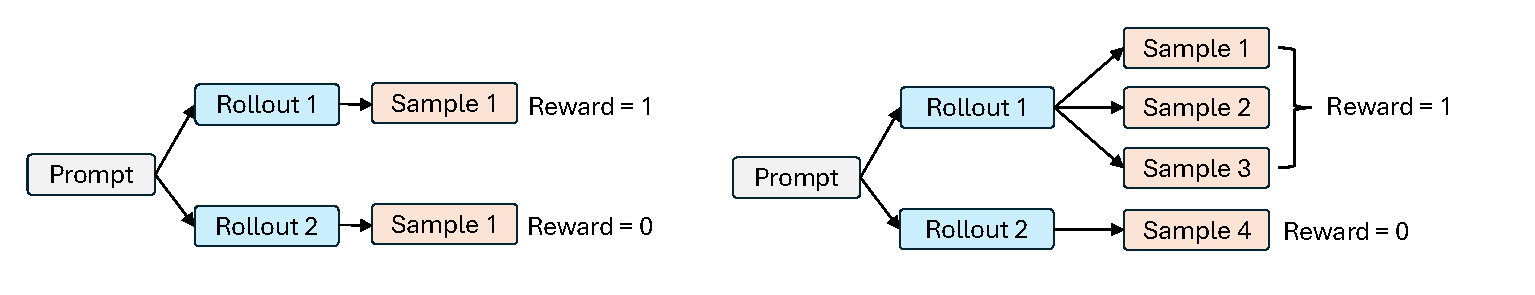
\includegraphics[width=\linewidth]{figures/agl-lite-reward.pdf}
  \caption{传统智能体 RL 中每次 rollout 是一个训练样本（\emph{左}），对比\add{\harl{}}中一次 rollout 可展开为继承其奖励的动态数量样本（\emph{右}）。}
  \label{fig:rollout-sample}
\end{figure}

我们认为 rollout 级优势是更合理的选择，理由如下。重分词是偶发现象，优势分配不应仅仅因为重分词恰巧把一次 rollout 拆成更多样本而改变。同理，子智能体派生与上下文摘要压缩是脚手架的内部操作，不应被允许改变整个组的基线。如何在一次 rollout 的样本之间设计更好的信用分配，仍有待未来工作。

\subsection{损失归一化}
\label{subsec:loss-normalization}

动态样本数也使损失归一化成为不平凡的选择。考虑一个包含 $R$ 次 rollout 的训练批次，其中 rollout $\rho$ 产生 $N_\rho$ 个样本，rollout $\rho$ 的第 $j$ 个样本有 $L_{\rho,j}$ 个响应 token，逐 token 损失为 $\ell_{\rho,j,t}$（$t=1,\ldots,L_{\rho,j}$）。多数框架直接沿用传统智能体 RL 的样本级归一化。第一种是 DAPO~\cite{dapo} 使用的 token 均值损失，对批次内所有 token 求和并按响应 token 总数归一化：
\begin{equation}
  \mathcal{L}_{\mathrm{token\text{-}mean}}
  = \frac{\sum_{\rho=1}^{R}\sum_{j=1}^{N_\rho}\sum_{t=1}^{L_{\rho,j}}
    \ell_{\rho,j,t}}
    {\sum_{\rho=1}^{R}\sum_{j=1}^{N_\rho} L_{\rho,j}}.
  \label{eq:token-mean}
\end{equation}
第二种是 GRPO~\cite{deepseekmath} 使用的序列均值-token 均值损失，先在每个样本内取均值，再对所有样本的样本均值均匀平均：
\begin{equation}
  \mathcal{L}_{\mathrm{seq\text{-}mean}}
  = \frac{1}{\sum_{\rho=1}^{R} N_\rho}
    \sum_{\rho=1}^{R}\sum_{j=1}^{N_\rho}
    \frac{1}{L_{\rho,j}}\sum_{t=1}^{L_{\rho,j}} \ell_{\rho,j,t}.
  \label{eq:seq-mean}
\end{equation}
slime~\cite{slime} 实现了 rollout 级 token 均值损失，先将一次 rollout 的所有响应 token 汇总，再在 rollout 之间均匀平均：
\begin{equation}
  \mathcal{L}_{\mathrm{rollout\text{-}mean}}
  = \frac{1}{R}\sum_{\rho=1}^{R}
    \frac{\sum_{j=1}^{N_\rho}\sum_{t=1}^{L_{\rho,j}} \ell_{\rho,j,t}}
    {\sum_{j=1}^{N_\rho} L_{\rho,j}}.
  \label{eq:rollout-mean}
\end{equation}

我们在图~\ref{fig:loss-normalization} 中给出更具体的例子。假设一个批次包含三次 rollout：Rollout A 产生两个样本 $A_1$ 与 $A_2$，响应长度分别为 50 与 100；Rollout B 产生三个样本 $B_1$、$B_2$ 与 $B_3$，每个响应长度 30；Rollout C 产生单个样本 $C_1$，响应长度 40。令 $A_1,A_2,B_1,B_2,B_3,C_1$ 同时表示各样本内逐 token 损失之和，即 $A_1=\sum_t \ell_{A,1,t}$，以此类推。则：
\begin{itemize}
  \item $\mathcal{L}_{\mathrm{token\text{-}mean}}
  = (A_1+A_2+B_1+B_2+B_3+C_1)/(50+100+30+30+30+40)$。
  \item $\mathcal{L}_{\mathrm{seq\text{-}mean}}
  = \tfrac{1}{6}(A_1/50+A_2/100+B_1/30+B_2/30+B_3/30+C_1/40)$。
  \item $\mathcal{L}_{\mathrm{rollout\text{-}mean}}
  = \tfrac{1}{3}\bigl((A_1+A_2)/(50+100)+(B_1+B_2+B_3)/(30+30+30)+C_1/40\bigr)$。
\end{itemize}

\begin{figure}[t]
  \centering
  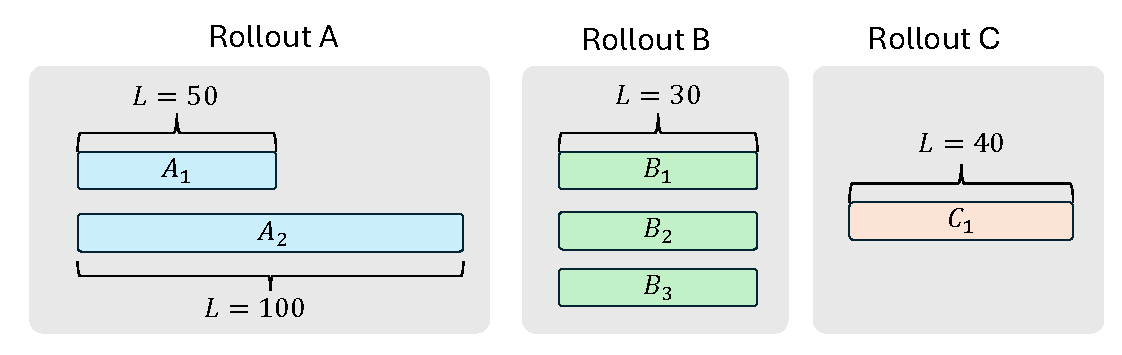
\includegraphics[width=0.65\linewidth]{figures/agl-lite-rollout-sample.pdf}
  \caption{一个包含三次 rollout、样本数与响应长度各异的示例批次。}
  \label{fig:loss-normalization}
\end{figure}

对损失归一化，我们持与优势计算相同的观点：样本数量不应被允许影响梯度归一化，因为它常由重分词等偶然因素驱动。在此观点下，式~\ref{eq:seq-mean} 的序列均值-token 均值损失是有问题的：它随单个 rollout 恰好产生的样本数而变化，总体上给样本更多的 rollout 不成比例的高权重。因此我们认为式~\ref{eq:token-mean} 的 token 均值损失与式~\ref{eq:rollout-mean} 的 rollout 级 token 均值损失在理论上更合理。但实践中我们发现 token 均值损失对长序列敏感：当批次中出现许多长负样本时，可能在训练后期引发不稳定。因此我们偏好式~\ref{eq:rollout-mean} 的 rollout 级 token 均值损失。

\subsection{训练后端复杂度}

动态样本数也使与训练后端的接口复杂化。一批 rollout 的样本数量与长度只有在脚手架执行与样本构建之后才能确定；相比之下，训练 GPU 数量与数据/张量/流水线并行配置在整个训练期间通常保持固定。后端因此必须在每次迭代将可变负载映射到固定 worker 集合上。

\add{样本构建之后，后端可将结果序列展平为物理张量批次，但这一变换必须保留其统计来源。尤其地，每条序列都应保留其 rollout 标识与 prompt 组标识：
\begin{equation}
  \mathcal{B}_{\mathrm{train}}
  =
  \bigcup_{\rho \in \mathcal{B}_{\mathrm{rollout}}}
  \left\{
    \bigl(S_{\rho,j},\rho,g_\rho\bigr)
    \;\middle|\;
    1 \le j \le N_\rho
  \right\},
\end{equation}
其中 $S_{\rho,j}$ 是由 rollout $\rho$ 构造的第 $j$ 条序列，$g_\rho$ 标识由同一 prompt 采样的一组 rollout。展平只改变物理表示，不得改变 rollout 归属，也不得让某次 rollout 仅仅因为产生了更多序列而获得额外统计权重。}

\add{rollout 边界还约束批次调度。基于行的张量批次、数据并行切分与小批次调度无法仅凭 prompt 或 rollout 数量提前规划，因为 $N_\rho$ 只有在执行后才知道。此外，同一次 rollout 的序列应保持在同一次优化器更新中——把它们拆分到不同更新中，会让一次 rollout 的不同部分在不同策略版本下被评估，引入 rollout 内策略偏差。后端因此必须在固定 worker 之间平衡 token 负载，同时保留这些 rollout 级统计与更新边界。}

\section{系统设计}
\label{sec:system-design}

\add{当训练器与智能体脚手架解耦后，没有任何单一进程拥有完整的 rollout 生命周期：训练器拥有模型推理与优化，脚手架拥有上下文构建、控制流、工具使用与环境交互。智能体执行可能远程运行、超出任何单次 API 请求或 worker 进程的生命周期，且可能独立于训练进程失败。要将这一架构落地，需要一个轻量控制面来协调持久化 rollout 状态、外部执行、部分失败与资源使用，同时不把脚手架逻辑拉回训练器。}

\add{Agent Lightning v1.0 围绕声明式 rollout 抽象与调和循环（reconciliation loop）构建这一控制面。训练器通过 API 网关声明 rollout——网关是生命周期状态与只追加事件的唯一事实来源。Rollout 控制器持续将这一状态与运行于 Kubernetes Job 或本地进程的智能体执行进行调和。这种分离使 Kubernetes 成为可替换的执行后端，而非 rollout 抽象本身的一部分。}

\add{同一控制面还提供了跨服务边界的显式可靠性与可观测性语义。控制面操作幂等，生成尝试被显式记录与裁决，rollout 标识将模型请求、奖励、自定义事件与执行日志关联为一条诊断记录。最后，API 网关协调共址异步 RL 期间的推理准入，允许 rollout 与权重更新在无需向外部脚手架暴露相位切换的情况下分时共享同一 GPU 池。}

如图~\ref{fig:teaser} 所示，Agent Lightning v1.0 通过三个组件连接训练集群（运行模型推理与训练的 GPU 集群）与智能体执行集群。API 网关是一个 API 服务，存储 rollout、模型与事件，并将来自智能体脚手架的 LLM 调用转发到训练器注册的模型端点。Rollout 控制器在 Kubernetes 集群（或本地进程池）之上管理智能体执行，从 API 网关轮询 rollout 并启动相应智能体任务。定制化训练器基于 VERL~\cite{hybridflow} 构建，向 API 网关注册 rollout，等待 Rollout 控制器驱动其完成，然后取回其记录的事件组装训练样本。经由这一链路，训练器只创建 rollout 与收集轨迹；任何脚手架只需将其 LLM 端点切换到代理即可接入；训练与执行资源可以独立供给，甚至运行在不同地点。

Agent Lightning v1.0 的设计追求尽可能简单：整个系统约 3500 行代码实现，每个组件职责清晰。Agent Lightning v1.0 还内置了针对第~\ref{sec:challenges} 节挑战的设计选择，如 rollout 级奖励与优势计算、rollout 级损失归一化。

我们在附录~\ref{sec:appendix-system-design} 中详细描述每个组件，下文重点介绍若干特性。

\subsection{共址异步 RL}

智能体 RL 中，同步 RL 训练很慢：批次内所有 rollout 必须完成才能进行训练步更新，训练步必须等待批次中最慢的 rollout，使大量 GPU 空闲。AReaL~\cite{areal} 提出的异步 RL 将 rollout 与更新拆分到两个独立的机器池、各自占用不同 GPU，从而在更新运行时 rollout GPU 保持工作，解决了 GPU 空闲问题。但我们发现这总体上需要更多 GPU，对资源有限的小团队而言要求过高；且需要分别管理 rollout 队列与更新队列，实践中两个队列进度可能不同，管理更复杂。

\begin{figure}[t]
	\centering
	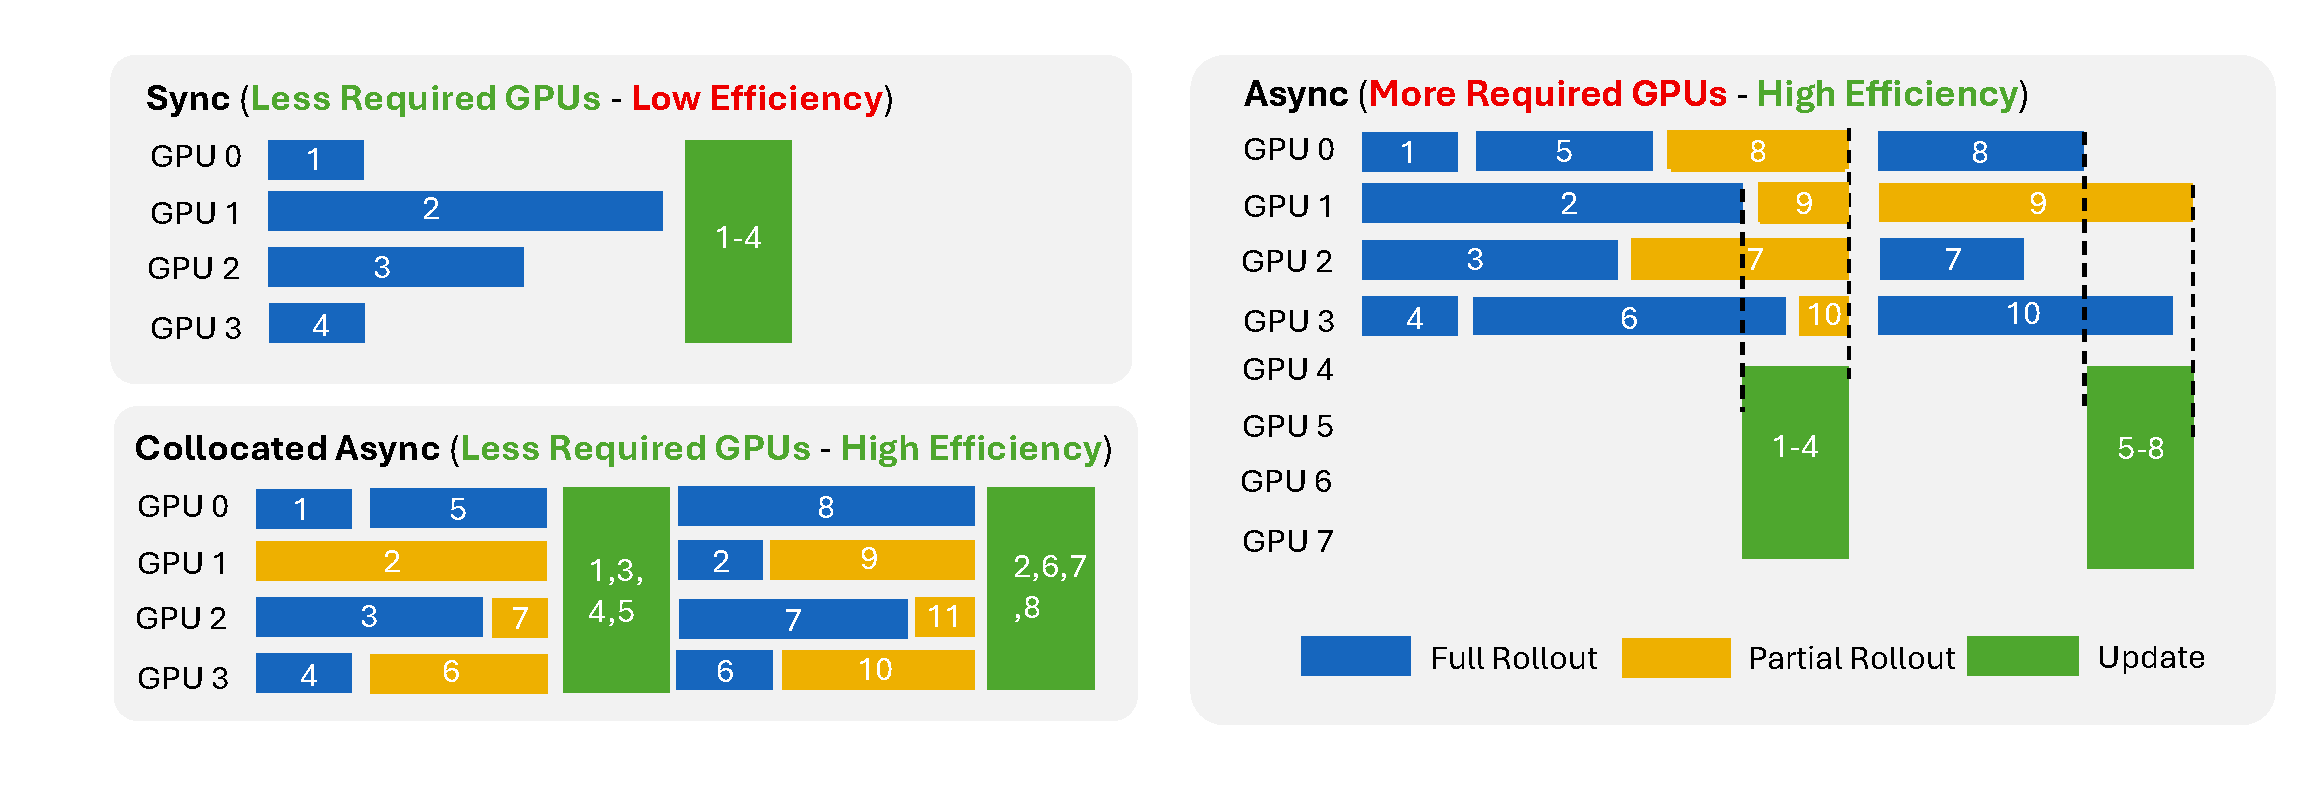
\includegraphics[width=\linewidth]{figures/agl-lite-async.pdf}
	\caption{同步 RL、异步 RL 与本文的共址异步 RL。共址异步 RL 在 rollout 与更新之间共享同一批 GPU，同时避免等待最慢的 rollout。}
	\label{fig:collocated-async}
\end{figure}

我们转而提出\emph{共址异步（collocated async）}，如图~\ref{fig:collocated-async} 所示。共址异步 RL 中，rollout 与权重更新共享同一 GPU 池。一旦收集到足够的 rollout 数据，更新步即开始。API 网关同时停止接受新请求并等待当前请求完成；此后若有新请求到达，网关将其暂停，直至系统重新进入 rollout 相位。因此，相位切换对智能体脚手架不可见。

共址异步让同一批 GPU 在 rollout 与训练之间分时共享，相比异步 RL 使用更少 GPU，同时避免等待最慢的 rollout。实验中，共址异步 RL 相比同步 RL 端到端加速约 2 倍，且使用更少 GPU。

\subsection{网络问题}

在\add{\harl{}}中，智能体与训练引擎分离，由此产生网络问题：两侧之间的调用经由网络传输，并非总是可靠。受影响的有两类调用：训练器或 Rollout 控制器到 API 网关的调用，以及智能体脚手架经代理到 LLM 推理端点的调用。两者都可能遭遇网络中断，调用方通常在失败后重试。我们用两项措施解决。

\paragraph{幂等的 API 网关端点。}我们将每个 rollout API 网关端点设计为幂等：重复同一调用任意次与调用一次效果相同。调用方因此在网络失败后可自由重试，无需担心重试本身破坏状态。

\paragraph{重复 LLM API 调用的去重。}重试的 LLM API 调用无法用同样方式幂等化，因为每次重试都是一次新的生成请求，可能返回不同响应。作为替代，定制化训练器在组装训练样本时对共享同一 prompt 的 \texttt{model\_request} 事件去重：若一次 rollout 记录了多个 prompt 相同的调用，只保留最后一次（最新）调用，丢弃更早的、对应重试或被取代的调用。

\subsection{Kubernetes 集成}

RL 训练的 rollout 阶段需要大量智能体并发运行，需要可观的计算资源。现有\add{\harl{}}框架普遍转向商业沙箱服务来满足这一需求：如 verl Uni-Agent~\cite{uniagent} 在 Modal Sandbox 与 Volcano veFaas 等托管沙箱上启动智能体执行，slime~\cite{slime} 依赖 E2B。这些服务提供便捷的开箱即用沙箱，但在 RL 训练规模下可能昂贵。

Agent Lightning v1.0 转而通过 Rollout 控制器直接在 Kubernetes 集群上运行智能体。每次智能体执行被调度为标准 Kubernetes Job，用户可完全依赖自托管或本地算力，而非商业沙箱提供商。这避免了商业沙箱服务的持续成本，并保持整个训练栈开源。

\subsection{监控}

训练期间，我们发现智能体自身可能出现问题，如奖励黑客、不良智能体行为与网络连接问题。人工检查 rollout 来发现这些问题很不方便，因此定制化训练器内置了监控系统，记录训练与验证 rollout 及 Kubernetes 的 pod 级日志，详见附录~\ref{sec:appendix-system-design}。该系统使我们能用 AI 智能体自动识别此类问题——我们确实借此发现了若干奖励黑客实例，见第~\ref{subsec:reward-hacking} 节。

\section{实验}

我们在三种实际的智能体训练场景中评估 Agent Lightning v1.0：搜索、通用指令遵循与编程。我们沿用 Search-R1~\cite{searchr1} 的实验设置训练搜索智能体，沿用 LLM-in-Sandbox~\cite{llminsandbox} 的设置训练通用指令遵循智能体。对编程智能体，我们从 SWE-smith~\cite{swesmith} 构建训练数据。

我们发现现有框架很少提供完整、可复现的编程智能体训练示例，可能源于数据清洗复杂、环境搭建困难与所需算力巨大。因此我们聚焦编程智能体，详细描述其训练过程，目标是提供一个完整可复现、仅需适量资源的示例。

\subsection{搜索智能体}

我们沿用 Search-R1~\cite{searchr1} 的实验设置，训练一个将推理与搜索引擎查询交织、利用检索到的段落回答知识密集问题的搜索智能体。策略模型为 Llama-3.2-3B-Instruct~\cite{llama3}，用 GRPO~\cite{deepseekmath} 优化。在 HotpotQA~\cite{hotpotqa} 训练集上训练。评估时，从 HotpotQA、2WikiMultiHopQA~\cite{2wikimultihopqa}、MuSiQue~\cite{musique}、Bamboogle~\cite{bamboogle}、TriviaQA~\cite{triviaqa} 与 Natural Questions~\cite{naturalquestions} 各采样 50 个样本。训练批次大小 512，每个 prompt 采样 4 次 rollout，每 10 个训练步评估一次。奖励指标为精确匹配（EM）。

图~\ref{fig:search-r1-training} 总结了训练动态。平均训练奖励稳步上升。验证集奖励从 25.1\% 提升至 41.7\%，绝对提升 16.6\%。

\begin{figure}[t]
  \centering
  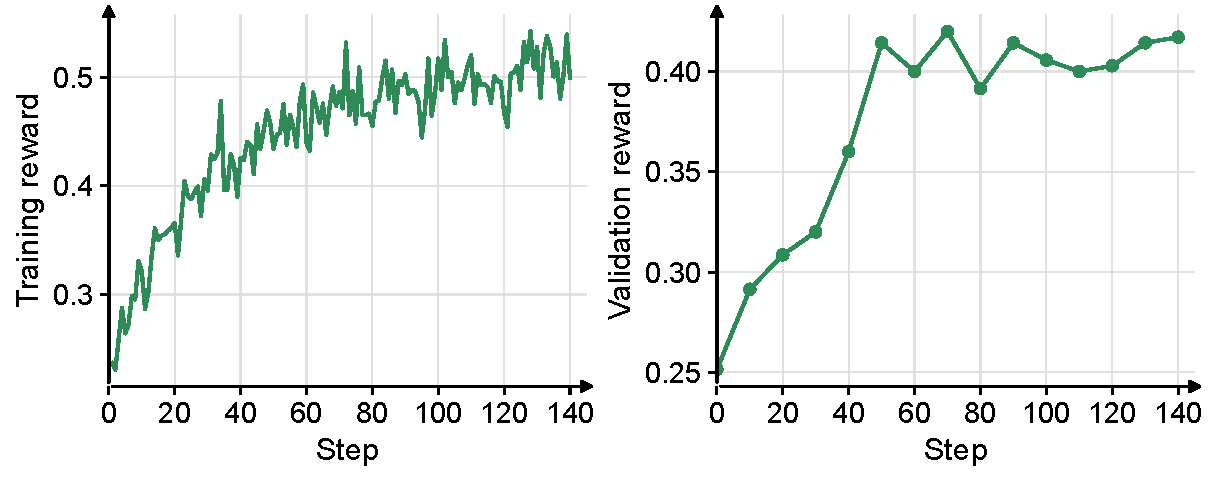
\includegraphics[width=0.65\textwidth]{figures/search-r1-metrics.pdf}
  \caption{搜索智能体训练动态。从左到右：平均训练奖励与平均验证奖励。}
  \label{fig:search-r1-training}
\end{figure}

\subsection{通用指令遵循智能体}

我们沿用 LLM-in-Sandbox~\cite{llminsandbox} 的实验设置训练通用指令遵循智能体。该智能体通过计算机沙箱访问外部资源、管理文件并执行代码，解决多样化的非编程任务。使用原作者提供的智能体脚手架。策略模型为 Qwen3-4B-Instruct-2507~\cite{qwen3}，用 RLOO~\cite{rloo} 优化。使用 Instruction Pre-Training~\cite{instructionpretraining} 发布的数据集，按 80\%/20\% 划分训练与评估。训练批次大小 8，每个 prompt 采样 8 次 rollout，每 20 个训练步评估一次。

图~\ref{fig:llm-in-sandbox-training} 显示批次级训练奖励噪声较大，而验证奖励呈现清晰的上升趋势：从 51.9\% 提升至 70.2\%，绝对提升 18.3\%。

\begin{figure}[t]
  \centering
  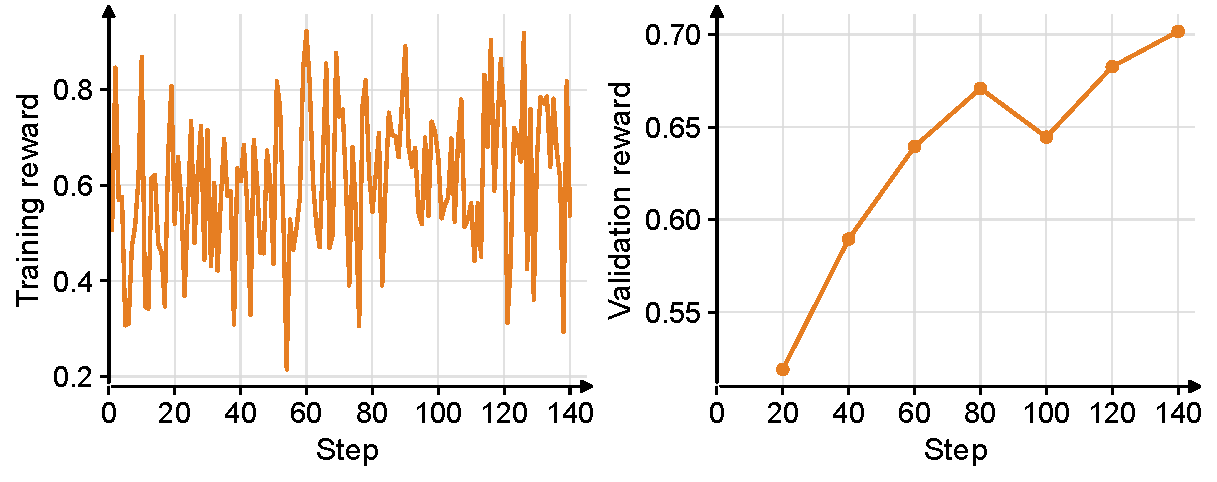
\includegraphics[width=0.65\textwidth]{figures/llm-in-sandbox-metrics.pdf}
  \caption{通用指令遵循智能体训练动态。从左到右：平均训练奖励与平均验证奖励。}
  \label{fig:llm-in-sandbox-training}
\end{figure}

\subsection{编程智能体}

我们基于 Qwen3.5-9B~\cite{qwen35}，使用 SWE-smith 数据集~\cite{swesmith} 派生的任务训练编程智能体。使用 mini-SWE-agent~\cite{minisweagent} 作为智能体脚手架，与仓库环境交互、执行命令并产出代码修改。为获得可靠的训练信号，我们应用详细的数据过滤管线，引入防奖励黑客保护措施，并实现健壮编程智能体训练所需的额外措施。下面描述这些实现细节。

\subsubsection{数据集预处理与过滤}

SWE-smith 是一个大规模可执行软件工程任务数据集，通过向真实 Python 仓库引入 bug 构建而成。它包含来自 128 个仓库的 59,136 个任务，附问题陈述、代码补丁与验证解法的测试~\cite{swesmith}。其 Docker 镜像仅占 295~GB~\cite{swesmith}，远小于 R2E-Gym~\cite{r2egym} 所需的 4~TB 与 SWE-Gym~\cite{swegym} 所需的 6~TB。

对每个任务，SWE-smith 先将仓库切换到对应问题分支，要求编程智能体修改代码库，然后运行任务专属测试套件判断提交的修改是否解决问题。

我们在发布数据中发现以下问题：
\begin{itemize}
  \item 59,136 条记录中有 18,033 条问题陈述为空。
  \item 1,265 条记录对应的问题分支在所提供 Docker 镜像中缺失。
  \item 部分任务需要大规模测试套件。例如 \texttt{python-jsonschema} 需要执行 7,000 多个测试，消耗大量 CPU 与内存。
\end{itemize}

因此我们移除问题陈述为空、问题分支缺失或测试数超过 200 的任务。剩余任务的难度分布仍然高度偏斜、训练信号有限，因此我们额外应用基于模型的难度过滤：对每个候选任务用 Qwen3.5-9B 运行四次——四次 rollout 全部解决的任务被移除，成功与失败并存的任务被保留，得到约 5,000 个样本。为避免结果集过于简单，我们额外采样 1,000 个四次 rollout 全部失败的任务。最终划分包含约 6,000 个训练样本与 400 个测试样本。

\subsubsection{防止奖励黑客}
\label{subsec:reward-hacking}

训练期间，我们观察到若干奖励黑客行为——智能体绕过预期的解题过程直接获取参考源代码：
\begin{enumerate}
  \item 使用 Git 历史定位正确提交。
  \item 使用 \texttt{wget} 或 \texttt{curl} 从 GitHub 获取上游源代码。
  \item 使用 \texttt{pip} 下载软件包源代码。
  \item 使用 Python 网络库（如 \texttt{urllib}）下载源代码。
\end{enumerate}

我们引入两道防护。第一，禁用 Git 命令并向智能体隐藏 \texttt{.git} 目录，阻止其检查提交历史。第二，强制 Kubernetes 网络策略，阻断一般出站网络访问，只允许连接显式白名单服务。两项措施共同要求智能体仅凭问题陈述与本地信息解题。

\subsubsection{训练动态}

\begin{figure}[t]
  \centering
  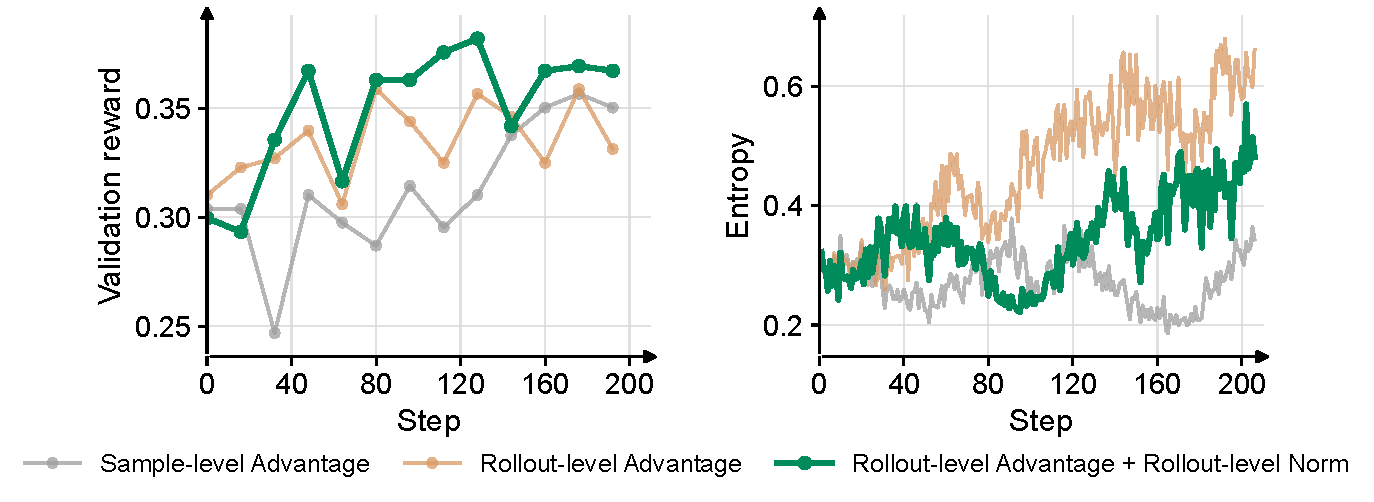
\includegraphics[width=0.75\textwidth]{figures/smith-ablation-metrics.pdf}
  \caption{样本级优势、rollout 级优势与 rollout 级优势 + rollout 级归一化三种设置的编程智能体训练动态。左：验证奖励。右：策略熵。}
  \label{fig:smith-ablation-training}
\end{figure}

\begin{figure}[t]
  \centering
  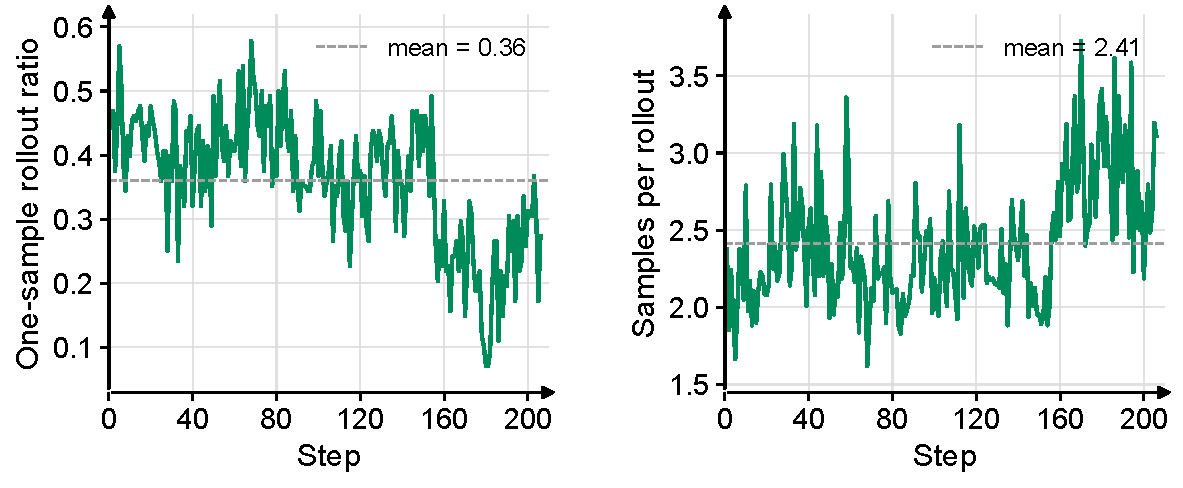
\includegraphics[width=0.75\textwidth]{figures/smith-merge-sample-metrics.pdf}
  \caption{rollout 级优势 + rollout 级归一化训练的 rollout 合并行为。左：恰好产生一个训练样本的 rollout 占比。右：每次 rollout 产生的平均训练样本数。虚线标记训练全程均值。}
  \label{fig:smith-merge-sample-metrics}
\end{figure}


如第~\ref{sec:challenges} 节所述，由于一次 rollout 的样本数常由重分词等偶然因素驱动，优势计算（第~\ref{subsec:advantage-calculation} 节）与损失归一化（第~\ref{subsec:loss-normalization} 节）都应在 rollout 层面而非样本层面计算。我们在编程智能体训练中对比三种设置验证这一设计选择，三者均使用相同的底层 GRPO 目标：
\begin{itemize}
  \item \emph{样本级优势}：样本级优势 + 式~\ref{eq:token-mean} 的 token 均值损失；
  \item \emph{rollout 级优势}：仅将优势计算切换到 rollout 级，保留 token 均值损失；
  \item \emph{rollout 级优势 + rollout 级归一化}：进一步将 token 均值损失替换为式~\ref{eq:rollout-mean} 的 rollout 级 token 均值损失。
\end{itemize}
图~\ref{fig:smith-ablation-training} 对比三种设置。最后一种变体获得最高的验证奖励：第 128 步达到 38.2\%，相比之下基线为 35.0\%，仅修复 rollout 优势时为 33.1\%。其策略熵增长也更慢、训练全程比仅修复 rollout 优势的变体更稳定。这些结果表明，损失归一化在提升验证奖励的同时控制了修正后的 rollout 优势带来的熵增。我们还在 SWE-bench Verified~\cite{swebench} 上评估了 rollout 级优势 + rollout 级归一化检查点：第 208 步从 41.8\% 提升至 56.4\%。由于编程智能体轨迹长度差异很大，rollout 级优势变体会尽可能将轨迹合并为训练行以减少填充浪费，由此产生动态的每-rollout 训练样本数：平均仅 36\% 的 rollout 保持为单一完全合并行，每次 rollout 平均产生 2.41 个训练样本（图~\ref{fig:smith-merge-sample-metrics}）。

\section{相关工作}

传统 RL 框架如 verl~\cite{hybridflow}、AReaL~\cite{areal} 与 slime~\cite{slime} 最初要求智能体循环直接实现在训练框架内部，遵循经典 ReAct 式~\cite{react} 马尔可夫形式——训练引擎拥有环境交互循环。这使得复用独立维护的智能体脚手架（如 mini-SWE-agent~\cite{minisweagent}、OpenHands~\cite{openhands}、OpenCode~\cite{opencode}、Claude Code~\cite{claudecode}、Codex~\cite{codex}、OpenClaw~\cite{openclaw} 与 Hermes~\cite{hermes}）十分困难，因为每个都需要在训练栈中重新实现。我们最初的 Agent Lightning~\cite{agentlightning} 工作提出了解耦架构，转而通过 LLM 端点将任意智能体脚手架接入 RL 训练；这种基于代理的方式此后被 verl Uni-Agent~\cite{uniagent}、AReaL 2.0~\cite{areal2}、slime v0.3.0~\cite{slime} 与 Polar~\cite{polar} 采纳。如第~\ref{sec:challenges} 节所述，这些框架在重分词、优势计算与损失归一化（每次 rollout 产生动态数量训练样本）上做出不同甚至相互冲突的设计选择，并普遍依赖商业沙箱服务（如 Modal Sandbox、Volcano veFaas 与 E2B）大规模执行智能体。Agent Lightning v1.0 则完全运行在自托管 Kubernetes 集群上，整个系统约 3500 行代码实现，为研究这些设计选择提供了紧凑透明的试验平台。我们分别在 Search-R1~\cite{searchr1}、LLM-in-Sandbox~\cite{llminsandbox} 与 SWE-smith~\cite{swesmith} 的搜索智能体、指令遵循与编程智能体设置上验证了它。

\section{结论}

我们刻画了\emph{\add{\harl{}}}这一范式——部署时智能体脚手架（而非训练引擎）拥有环境交互循环——并识别了由此产生的重分词、优势计算、损失归一化与训练后端调度挑战。我们提出 Agent Lightning v1.0：一个约 3500 行的框架，支持任意智能体脚手架，并内置我们对这些挑战的 rollout 级设计选择。我们在搜索、指令遵循与编程智能体上验证了它，并发布完整数据管线与防奖励黑客保护措施——\add{仅靠 RL 即用约 6K 训练样本将 Qwen3.5-9B 在 SWE-bench Verified 上从 41.8\% 提升至 56.4\%，提升 14.6 个百分点}。我们发布完整代码库与脚本，促进可复现的\add{\harl{}}研究。


\clearpage
\bibliographystyle{unsrtnat}
\bibliography{reference}

\clearpage
\appendix
\section{详细系统设计}
\label{sec:appendix-system-design}

本附录详细描述第~\ref{sec:system-design} 节介绍的 Agent Lightning v1.0 三个组件：API 网关、Rollout 控制器与定制化训练器。

\subsection{API 网关}

API 网关是 Agent Lightning v1.0 的中心组件，刻意保持轻量：一个有状态服务，存储 rollout、模型与事件，并通过最小 API 暴露它们。图~\ref{fig:api-gateway-schema} 总结这些对象及其关系。

\begin{figure}[t]
	\centering
	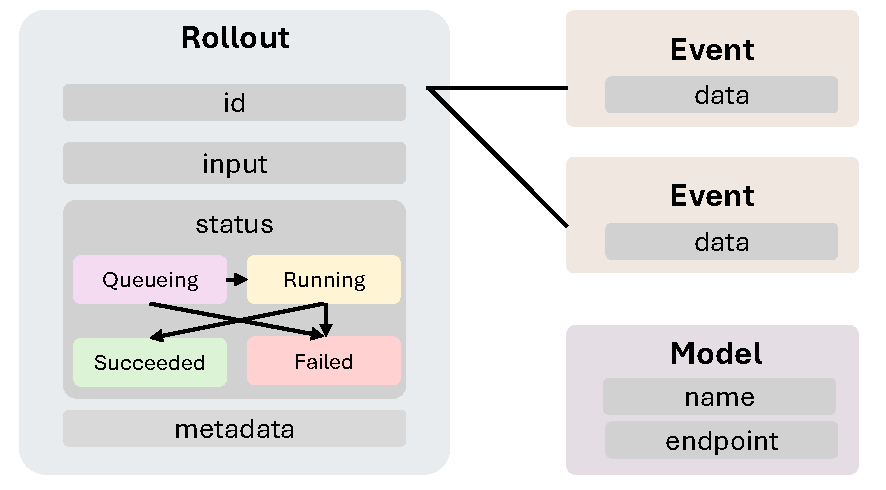
\includegraphics[width=0.5 \linewidth]{figures/agl-lite-schema.pdf}
	\caption{API 网关存储的对象。}
	\label{fig:api-gateway-schema}
\end{figure}

\paragraph{Rollout。}
一次\emph{rollout} 是一次智能体执行，由唯一 rollout ID 标识。它存储输入（源自训练样本）、状态与用户自定义元数据。状态遵循图~\ref{fig:api-gateway-schema} 中的状态机：\texttt{queuing}、\texttt{running} 与终止状态 \texttt{succeeded}、\texttt{failed}。rollout 与训练样本并非一一对应：例如 GRPO~\cite{deepseekmath} 从同一样本生成多次独立 rollout，各自拥有独立 ID 与轨迹。

\paragraph{模型。}
一个\emph{模型}以其名称与地址标识一个 LLM 推理端点。训练器向 API 网关注册模型，网关随后将智能体脚手架请求路由至对应推理服务器。

\paragraph{事件。}
一个\emph{事件}向 rollout 附加任意数据。默认情况下，Agent Lightning v1.0 为每次 LLM 交互记录 \texttt{model\_request} 事件（prompt token ID、响应 token ID 与响应对数概率），并记录智能体通常在 rollout 结束时一次性上报标量奖励的 \texttt{reward} 事件。用户也可以定义自定义事件类型。

\medskip

表~\ref{tab:api-gateway-endpoints} 列出 API 网关的端点，分两类 API：rollout API 与代理 API。

\begin{table}[t]
	\centering
	\small
	\begin{tabular}{@{}lp{0.43\linewidth}p{0.42\linewidth}@{}}
		\toprule
		方法 & 端点 & 说明 \\
		\midrule
		POST & \path|/api/rollouts| & 批量创建 rollout。 \\
		GET & \path|/api/rollouts| & 列出 rollout，可按状态过滤。 \\
		GET & \path|/api/rollouts/{rollout_id}| & 获取单个 rollout。 \\
		PATCH & \path|/api/rollouts/{rollout_id}| & 更新 rollout 状态。 \\
		POST & \path|/api/rollouts/{rollout_id}/attempt/{attempt_id}/events| & 向 rollout 尝试追加事件。 \\
		GET & \path|/api/rollouts/{rollout_id}/events| & 读取 rollout 事件。 \\
		\midrule
		POST & \path|/api/models| & 注册模型端点。 \\
		DELETE & \path|/api/models| & 移除所有已注册模型端点。 \\
		POST & \path|/proxy/rollout/{rollout_id}/attempt/{attempt_id}/mode/{mode}/openai/v1/chat/completions| & 转发 OpenAI 兼容模型调用。 \\
		\bottomrule
	\end{tabular}
	\caption{API 网关端点。}
	\label{tab:api-gateway-endpoints}
\end{table}

\paragraph{Rollout API。}
训练器通过此 API 创建 rollout。Rollout 控制器轮询排队中的 rollout、启动智能体并在执行过程中更新其状态。奖励与其他用户自定义事件以同样方式上传。

\paragraph{代理 API。}
此 API 将来自智能体脚手架的 LLM 调用转发至训练器注册的模型端点。智能体脚手架只需将其 OpenAI 兼容客户端指向代理。由于代理路径嵌入了 rollout ID，每次调用都能自动归属到其 rollout。每次调用的 prompt token ID、响应 token ID 与对数概率被记录为 \texttt{model\_request} 事件，供训练器稍后导出训练。

这一简单 API 将 RL 训练与智能体执行完全解耦：训练器只创建 rollout 与收集轨迹；任何脚手架只需将其 LLM 端点切换到代理即可接入；训练与执行资源可以独立供给，甚至运行在不同地点。

\subsection{Rollout 控制器}

Rollout 控制器在 Kubernetes 之上管理智能体执行。如图~\ref{fig:rollout-controller} 所示，它定期从 API 网关获取活跃 rollout，启动相应智能体任务、监控它们，并通过网关 API 回报状态。其主要后端是 K8s 协调器（K8s Reconciler），面向开源 Kubernetes 集群；为便于调试，还提供面向本地进程池的本地协调器（Local Reconciler）。

\begin{figure}[t]
	\centering
	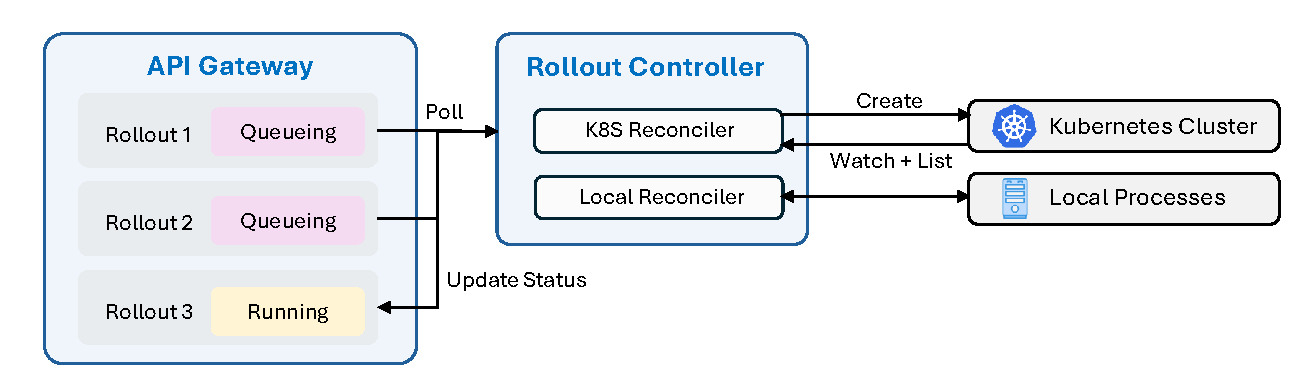
\includegraphics[width=\linewidth]{figures/agl-lite-controller.pdf}
	\caption{Rollout 控制器将 API 网关中的 rollout 状态与以 Kubernetes Job 或本地进程运行的智能体执行进行调和。}
	\label{fig:rollout-controller}
\end{figure}

\paragraph{K8s 协调器。}
对每个尚无对应 Kubernetes Job 的 \texttt{queuing} rollout，它依据用户提供的模板创建一个 Job。它监听 Kubernetes API 的 Job 更新，使终止状态低延迟传播；并周期性列举所有受管 Job 以恢复错过的监听事件——标准 Kubernetes 控制器模式。

\paragraph{本地协调器。}
它在本地进程池中启动智能体。由于直接持有进程句柄，仅周期性轮询即足够，无需单独监听机制。

\paragraph{状态一致性。}
API 网关的 rollout 状态是事实来源。从 Kubernetes 观察到的执行状态可能因网络失败或延迟更新而滞后。K8s 协调器只需在下一周期重试同步，两侧在通信恢复后收敛。这一设计只保证尽力而为的最终一致性。

\subsection{定制化训练器}

定制化训练器基于 VERL~\cite{hybridflow} 构建，在保持轻量设计的同时将训练后端接入 API 网关：每步为当前批次注册 rollout，等待其到达终止状态，然后取回其 \texttt{model\_request} 与 \texttt{reward} 事件并组装为训练样本。它由以下两个组件组成。

\paragraph{专用样本适配器。}
该适配器体现我们对第~\ref{sec:challenges} 节所述挑战的设计选择。
\begin{itemize}
	\item \textbf{样本合并。}我们让 API 网关尽可能简单：不维护服务端请求缓冲区，使训练与部署保持一致。适配器仅在后一次 prompt 是前一次请求与响应的精确 token 级前缀匹配时，才将两次相邻模型请求合并为一个训练样本。
	\item \textbf{优势计算。}适配器在 rollout 层面计算基线与优势，我们认为这是更合理的选择。
	\item \textbf{损失归一化。}适配器实现第~\ref{sec:challenges} 节讨论的 rollout 级 token 均值损失，使每次 rollout 无论样本数多少都携带相等权重。
\end{itemize}

\paragraph{轨迹监控。}
由于智能体训练可能产生奖励黑客、失控轨迹或静默失败，训练器暴露每次训练与验证 rollout 的输入、状态、模型请求、奖励、token/回合统计与自定义事件，执行日志保存在 Kubernetes 中，便于人工或借助 AI 智能体检查，诊断异常行为。


\end{document}
